%%=============================================================================
%% Resultaten
%%=============================================================================

\chapter{Resultaten}
\label{ch:resultaten}
%ResponseRelevancy  Scores the relevancy of the answer according to the given question. Answers with incomplete, redundant or unnecessary information is penalized. Score can range from 0 to 1 with 1 being the best.

%Faithfulness The Faithfulness metric measures how factually consistent a response is with the retrieved context. It ranges from 0 to 1, with higher scores indicating better consistency.

% AnswerCorrectness  Measures answer correctness compared to ground truth as a combination of factuality and semantic similarity.

%LLMContextRecall checkt in hoeverre de juiste info voor het antwoord ook effectief aanwezig was in de opgehaalde context. Hoe meer overlap tussen juiste antwoord en context, hoe hoger de score.  aka hoe goed het model zijn retrievalproces heeft aangestuurd.

Om de verschillende modellen te testen, worden meerdere scenario’s uitgevoerd.
Ten eerste wordt gebruikgemaakt van een testset met 10 vragen waarvan de informatie beschikbaar is in de documentatie. Van elk model wordt verwacht dat het op iedere vraag een concreet antwoord geeft. Deze antwoorden worden vervolgens geëvalueerd met behulp van het test framework \textit{Ragas}, waarbij vier verschillende meetcriteria worden toegepast.
\\[1em]
Het tweede testscenario bestaat uit het stellen van niet-triviale vragen waarvoor de informatie niet beschikbaar is in de documentatie. Dit scenario is vooral bedoeld om te onderzoeken of bepaalde modellen tekenen van hallucinaties vertonen.
\\[1em]
Als laatste worden enkele triviale vragen gesteld. Hierbij wordt getest of het model in staat is een juiste inschatting te maken door direct te antwoorden, zonder onnodige zoekopdrachten in de vectordatabase.

\section{Evaluatie 1: Documentatiegebaseerde vragen}

Elk model kreeg dezelfde vragenlijst te verwerken, waarbij de verwachte antwoorden zijn opgenomen in bijlage \ref{vragenlijst}.
De antwoorden die door de modellen zijn gegenereerd, zijn weergegeven in bijlage \ref{antwoordenlijst}.
In beide bijlagen zijn uit privacy overwegingen alle contactgegevens geanonimiseerd.
\\[1em]
Voor deze evaluatie wordt gebruikgemaakt van het test framework Ragas. Tijdens de testen wordt voor iedere vraag de volgende informatie verzameld: de gebruikersinput, de opgehaalde context, het antwoord van de LLM en het verwachte antwoord. Op basis van deze gegevens gebruikt Ragas zelf een LLM om de dataset te beoordelen. In dit geval werd als testmodel \textit{gemma3:4b} gekozen. Dit model biedt een goede balans tussen rekensnelheid, geheugengebruik en beoordelingskwaliteit. Hierdoor kon de evaluatie efficiënt worden uitgevoerd. Dit resulteert in een rapport waarin iedere vraag wordt beoordeeld op verschillende criteria.
\\[1em]
Iedere vraag werd beoordeeld op vier verschillende categorieën. De score per categorie variëren tussen 0 en 1, waarbij een score van 1 een volledig correct antwoord representeert.
\\[1em]
De vier gebruikte meetcriteria zijn \textit{Faithfulness}, \textit{Response Relevancy}, \textit{Answer Correctness} en \textit{Context Recall}. Het meetcriterium Faithfulness beoordeelt hoe consistent het antwoord is met de opgehaalde context. Response Relevancy kijkt naar hoe relevant het antwoord is ten opzichte van de vraag. Onvolledige of overbodige informatie leidt hierbij tot een lagere score. Answer Correctness beoordeelt hoe correct het antwoord is in vergelijking met het verwachte antwoord. Hierbij worden zowel feitelijke als semantische overeenkomsten meegenomen. Context Recall controleert in welke mate de benodigde informatie voor het antwoord aanwezig is in de opgehaalde context. Hoe groter de overlap tussen het juiste antwoord en de context, hoe hoger de score. Dit meetcriterium kijkt dus vooral naar hoe goed het model het ophaalproces aanstuurt.
\\[1em]
Bij sommige modellen en vragen traden tijdens het testen errors op. Dit hield in dat de documentatie ofwel niet werd opgehaald, ofwel foutief uit de vectordatabase kwam. Voor deze vragen werd vastgesteld dat de meetcriteria Faithfulness en Response Relevancy een score van nul kregen, terwijl Context Recall een perfecte één score werd toegekend. Om een realistischer beeld van de prestaties van de modellen te geven, werd voor deze vragen de Context Recall aangepast naar nul. Deze correctie werd toegepast voor Llama3.1 vraag vier en voor Qwen2.5 vragen vier, zeven en negen.
\\[1em]
%Vragen waar het model geen antwoord op kon bieden waren 1, 2, 7 en 10 Voor vragen 3, gaf het model wel een antwoord maar dit was niet in het geval van vraag 3 niet waarheidsgetrouw in het geval van vragen 5, lag het probleem eerder aan de documentatie die niet éénduidig was. Bij vraag 4 was er een error tijdens het RAG proces wat resulteerde in de slechte resultaten.
In tabel \ref{tab:resultaten_vragen_llama3.1} worden de resultaten van Llama3.1 weergegeven. Opvallend is dat de Response Relevancy in veel gevallen nul scoort, wat aangeeft dat de antwoorden van het model vaak niet relevant zijn voor de gestelde gebruikersvragen. Daarnaast blijft de score voor Answer Correctness over het algemeen laag. Dit valt deels te verklaren doordat het model voor een aantal vragen de nodige informatie niet kon vinden in de vectordatabase.
\\[1em]
Verder valt op dat het model vaak wel de juiste informatie in de context heeft, maar deze niet correct weet te gebruiken om tot het juiste antwoord te komen. Een duidelijk voorbeeld hiervan is vraag 10. Hier was de Context Recall een één, maar de Answer Correctness slechts 0.205. Het model gaf aan de vraag niet te kunnen beantwoorden, ondanks dat de benodigde informatie wel beschikbaar was in de context.

\begin{table}[H]
    \begin{tabular}{|l|c|c|c|c|}
        \hline
        \textbf{Vraag} & \textbf{Faithfulness} & \textbf{Response Relevancy} & \textbf{Answer Correctness} & \textbf{Context Recall} \\
        \hline
        Vraag 1 & 1.000 & 0.000 & 0.225 & 0.500 \\
        Vraag 2 & 0.333 & 0.000 & 0.221 & 0.000 \\
        Vraag 3 & 0.385 & 0.000 & 0.223 & 0.500 \\
        Vraag 4 & 0.000 & 0.000 & 0.174 & 0.000 \\
        Vraag 5 & 1.000 & 0.863 & 0.212 & 0.125 \\
        Vraag 6 & 0.667 & 0.920 & 0.477 & 1.000 \\
        Vraag 7 & 0.500 & 0.000 & 0.205 & 1.000 \\
        Vraag 8 & 0.714 & 0.000 & 0.408 & 1.000 \\
        Vraag 9 & 0.500 & 0.932 & 0.391 & 1.000 \\
        Vraag 10 & 0.333 & 0.000 & 0.205 & 1.000 \\
        \hline
    \end{tabular}
    \caption{Resultaten per vraag op de vier meetcriteria van het Llama3.1 model. De antwoorden blijken vaak niet relevant voor de vraag (Response Relevancy = 0), en de Answer Correctness blijft over het algemeen laag.}
    \label{tab:resultaten_vragen_llama3.1}
\end{table}

In tabel \ref{tab:resultaten_vragen_llama3.2} worden de resultaten van Llama3.2 weergegeven. Het meest opvallende resultaat is vraag zeven, waar het model zeer hoge scores behaalt op alle criteria en bijna een perfecte score bereikt voor Answer Correctness (0.991). Daarnaast laat het model, ondanks de kleinere modelgrootte, toch degelijke prestaties zien.
\\[1em]
Ook de resultaten voor vraag acht zijn opmerkelijk. Hier behaalt het model op bijna alle criteria een hoge score, met uitzondering van Answer Correctness. Dit verschil wordt veroorzaakt door de ambiguïteit in de opgehaalde documentatie. De bronnen boden geen eenduidig correct antwoord. Het door het model gegeven antwoord komt daardoor niet overeen met de ground truth, maar kan wel worden verantwoord op basis van de beschikbare documentatie.
\begin{table}[H]
    \centering
    \begin{tabular}{|l|c|c|c|c|}
        \hline
        \textbf{Vraag} & \textbf{Faithfulness} & \textbf{Response relevancy} & \textbf{Answer Correctness} & \textbf{Context Recall} \\
        \hline
        Vraag 1  & 0.500 & 0.894 & 0.485 & 0.500 \\
        Vraag 2  & 0.333 & 0.000 & 0.220 & 0.000 \\
        Vraag 3  & 0.800 & 0.000 & 0.219 & 0.500 \\
        Vraag 4  & 0.571 & 0.863 & 0.196 & 0.833 \\
        Vraag 5  & 0.625 & 0.000 & 0.205 & 0.125 \\
        Vraag 6  & 0.857 & 0.000 & 0.194 & 1.000 \\
        Vraag 7  & 0.917 & 0.860 & 0.991 & 1.000 \\
        Vraag 8  & 0.833 & 0.953 & 0.212 & 1.000 \\
        Vraag 9  & 0.429 & 0.883 & 0.631 & 0.375 \\
        Vraag 10 & 0.333 & 0.000 & 0.207 & 1.000 \\
        \hline
    \end{tabular}
    \caption{Resultaten per vraag op de vier meetcriteria van het Llama3.2 model. Opvallend is vraag zeven, waar het model bijna perfecte scores behaalt op alle criteria. Bij vraag acht werd vastgesteld dat ambiguïteit in de documentatie kan leiden tot een lage Answer Correctness, ondanks hoge scores op de andere criteria.}
    \label{tab:resultaten_vragen_llama3.2}
\end{table}

In tabel \ref{tab:resultaten_vragen_qwen2.5} worden de resultaten van Qwen2.5 weergegeven. Opvallend is dat de Response Relevancy vrijwel overal nul scoort en dat de Context Recall zeer laag is. De enige uitzondering is vraag zes, waar het model zowel de context correct ophaalt als een relevante respons genereert. Deze lage scores zijn deels het gevolg van errors tijdens het uitvoeren van het RAG-proces. Een andere reden is dat het model in sommige gevallen direct een antwoord formuleerde zonder eerst de vectordatabase te raadplegen. Ook blijft de score voor Answer Correctness voor de andere vragen relatief laag waardoor de prestaties van dit model niet overtuigend zijn.

\begin{table}[H]
    \begin{tabular}{|l|c|c|c|c|}
        \hline
        \textbf{Vraag} & \textbf{Faithfulness} & \textbf{Response relevancy} & \textbf{Answer Correctness} & \textbf{Context Recall} \\
        \hline
        Vraag 1  & 0.750 & 0.000 & 0.485 & 0.500 \\
        Vraag 2  & 0.500 & 0.000 & 0.226 & 0.000 \\
        Vraag 3  & 0.929 & 0.000 & 0.229 & 0.500 \\
        Vraag 4  & 0.000 & 0.000 & 0.174 & 0.000 \\
        Vraag 5  & 0.000 & 0.000 & 0.180 & 0.000 \\
        Vraag 6  & 1.000 & 0.871 & 0.469 & 1.000 \\
        Vraag 7  & 0.000 & 0.000 & 0.176 & 0.000 \\
        Vraag 8  & 0.000 & 0.000 & 0.179 & 0.000 \\
        Vraag 9  & 0.000 & 0.000 & 0.176 & 0.000 \\
        Vraag 10 & 0.667 & 0.000 & 0.216 & 0.000 \\
        \hline
    \end{tabular}
    \caption{Resultaten per vraag op de vier meetcriteria van het Qwen2.5 model. De Response Relevancy en Context Recall zijn vrijwel overal nul, met uitzondering van vraag zes waar het model zowel de context correct ophaalt als een relevante respons geeft. Over alle vragen blijft de Answer Correctness laag, wat duidt op matige prestaties van dit model.}
    \label{tab:resultaten_vragen_qwen2.5}
\end{table}


In tabel \ref{tab:resultaten_vragen_qwen3} worden de resultaten van Qwen3 weergegeven. Voor dit model valt op hoe hoog de Faithfulness is wat betekent dat het model zich goed houdt aan de informatie die het heeft opgehaald en bijgevolg minder geneigd is om hallucinaties te vertonen. Het model scoort voor vraag zeven zeer hoog op alle categorieën. De Answer Correctness blijft bij enkele vragen echter laag. Voor vragen één tot en met vier gaf het model aan geen antwoord te kunnen vinden in de context. Bij vraag vijf werd gedateerde informatie uit de vectordatabase opgehaald waardoor het antwoord niet overeenstemde met de ground truth. Voor vraag negen werd slechts een deel van het correcte antwoord uit de database gehaald. Op basis van de opgehaalde context besloot het model een andere chunk te gebruikten om een antwoord te genereren. Dit resulteert in een lage Answer Correctness met op hetzelfde moment een hoge Faithfulness en een vrij hoge Context Recall voor vraag negen.

\begin{table}[H]
    \begin{tabular}{|l|c|c|c|c|}
        \hline
        \textbf{Vraag} & \textbf{Faithfulness} & \textbf{Response Relevancy} & \textbf{Answer Correctness} & \textbf{Context Recall} \\
        \hline
        Vraag 1  & 1.000 & 0.000 & 0.216 & 0.500 \\
        Vraag 2  & 1.000 & 0.000 & 0.224 & 0.000 \\
        Vraag 3  & 1.000 & 0.000 & 0.220 & 0.250 \\
        Vraag 4  & 0.857 & 0.000 & 0.203 & 0.000 \\
        Vraag 5  & 0.636 & 0.867 & 0.211 & 0.125 \\
        Vraag 6  & 0.750 & 0.874 & 0.571 & 1.000 \\
        Vraag 7  & 1.000 & 0.906 & 0.989 & 1.000 \\
        Vraag 8  & 0.556 & 0.000 & 0.411 & 1.000 \\
        Vraag 9  & 1.000 & 0.000 & 0.340 & 0.625 \\
        Vraag 10 & 1.000 & 0.935 & 0.636 & 1.000 \\
        \hline
    \end{tabular}
    \caption{Resultaten per vraag voor het Qwen3 model waarbij opvalt dat Faithfulness hoog is en het model bij vraag zeven op alle meetcriteria hoge scores behaalt terwijl de Answer Correctness bij enkele vragen lager blijft door ontbrekende of gedateerde informatie.}
    \label{tab:resultaten_vragen_qwen3}
\end{table}


\subsection{Samenvatting}

Om de prestaties van de modellen per meetcriterium te vergelijken, worden in figuur~\ref{fig:vergelijking_metrics} vier staafdiagrammen weergegeven. Elk diagram toont de gemiddelde score van de verschillende modellen voor één specifiek meetcriterium.

\begin{figure}[H]
    \centering
    \begin{subfigure}{0.48\textwidth}
        \centering
        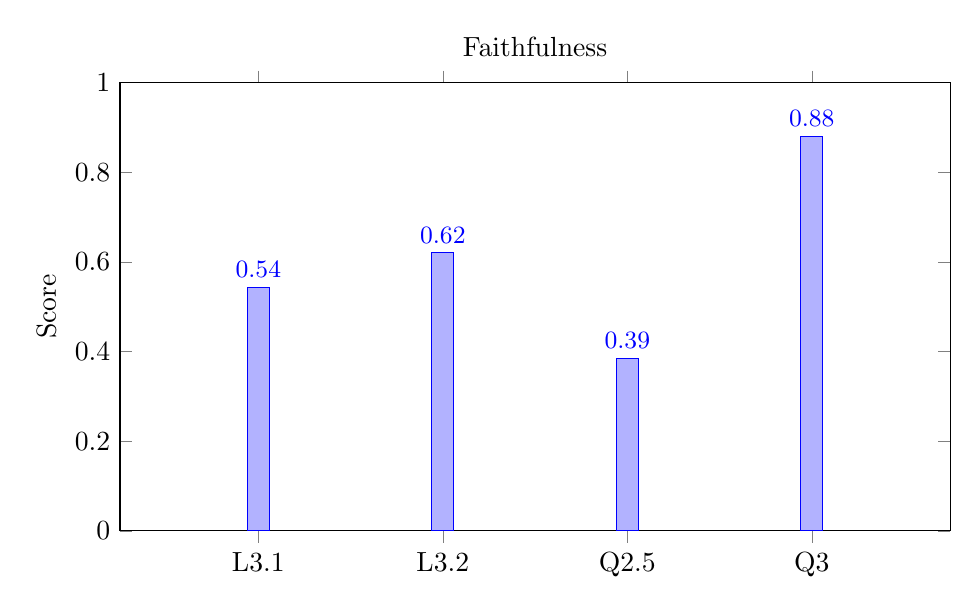
\begin{tikzpicture}
            \begin{axis}[
                ybar,
                ymin=0,
                ymax=1,
                bar width=8pt,
                width=\textwidth,
                height=0.6\textwidth,
                enlarge x limits=0.25,
                ylabel={Score},
                symbolic x coords={L3.1,L3.2,Q2.5,Q3},
                xtick=data,
                nodes near coords,
                nodes near coords align={vertical},
                every node near coord/.append style={font=\small},
                title={Faithfulness}
                ]
                \addplot coordinates {(L3.1,0.543) (L3.2,0.620) (Q2.5, 0.385) (Q3,0.880)};
            \end{axis}
        \end{tikzpicture}
    \end{subfigure}
    \hfill
    \begin{subfigure}{0.48\textwidth}
        \centering
        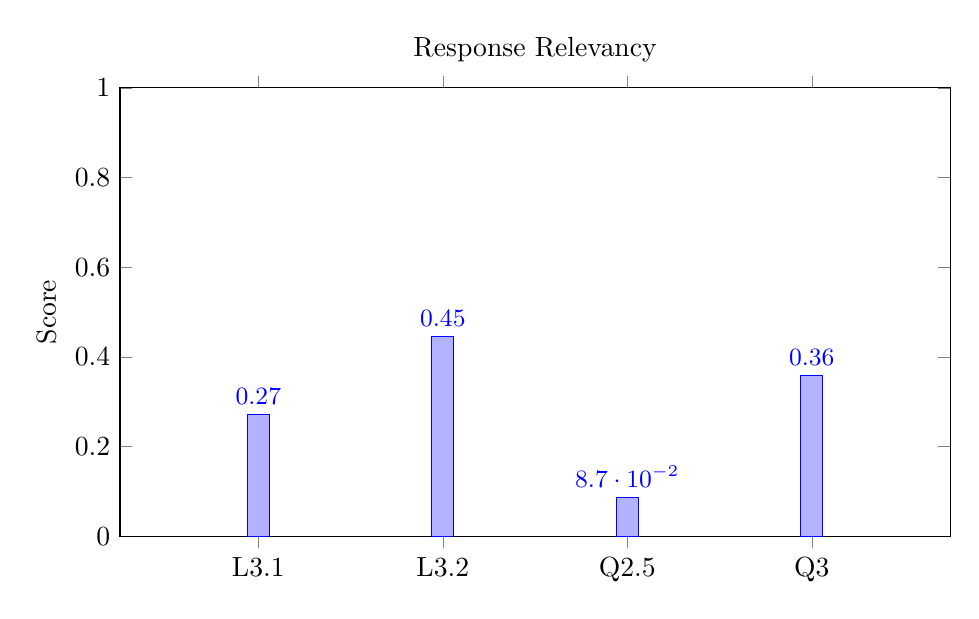
\begin{tikzpicture}
            \begin{axis}[
                ybar,
                ymin=0,
                ymax=1,
                bar width=8pt,
                width=\textwidth,
                height=0.6\textwidth,
                enlarge x limits=0.25,
                ylabel={Score},
                symbolic x coords={L3.1,L3.2,Q2.5,Q3},
                xtick=data,
                nodes near coords,
                nodes near coords align={vertical},
                every node near coord/.append style={font=\small},
                title={Response Relevancy}
                ]
                \addplot coordinates {(L3.1,0.272) (L3.2,0.445) (Q2.5,0.087) (Q3,0.358)};
            \end{axis}
        \end{tikzpicture}
    \end{subfigure}
    
    \vspace{1em}
    
    \begin{subfigure}{0.48\textwidth}
        \centering
        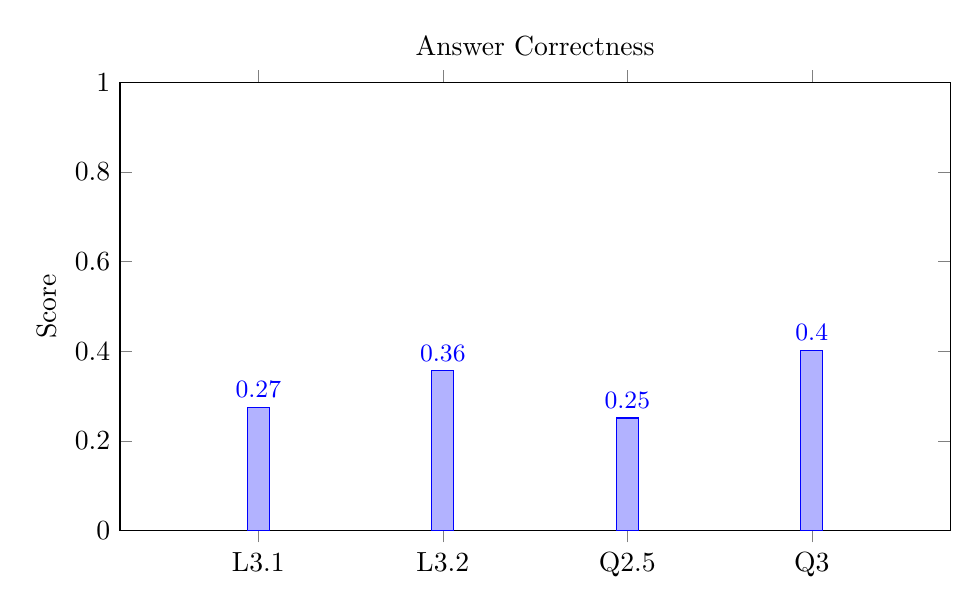
\begin{tikzpicture}
            \begin{axis}[
                ybar,
                ymin=0,
                ymax=1,
                bar width=8pt,
                width=\textwidth,
                height=0.6\textwidth,
                enlarge x limits=0.25,
                ylabel={Score},
                symbolic x coords={L3.1,L3.2,Q2.5,Q3},
                xtick=data,
                nodes near coords,
                nodes near coords align={vertical},
                every node near coord/.append style={font=\small},
                title={Answer Correctness}
                ]
                \addplot coordinates {(L3.1,0.274) (L3.2,0.356) (Q2.5,0.251) (Q3,0.402)};
            \end{axis}
        \end{tikzpicture}
    \end{subfigure}
    \hfill
    \begin{subfigure}{0.48\textwidth}
        \centering
        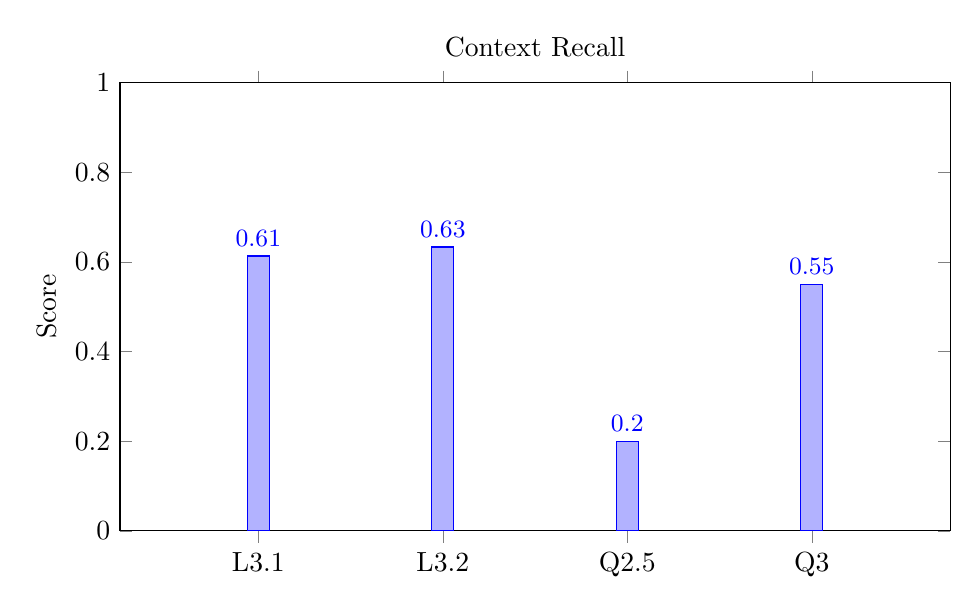
\begin{tikzpicture}
            \begin{axis}[
                ybar,
                ymin=0,
                ymax=1,
                bar width=8pt,
                width=\textwidth,
                height=0.6\textwidth,
                enlarge x limits=0.25,
                ylabel={Score},
                symbolic x coords={L3.1,L3.2,Q2.5,Q3},
                xtick=data,
                nodes near coords,
                nodes near coords align={vertical},
                every node near coord/.append style={font=\small},
                title={Context Recall}
                ]
                \addplot coordinates {(L3.1,0.613) (L3.2,0.633) (Q2.5,0.2) (Q3, 0.550)};
            \end{axis}
        \end{tikzpicture}
    \end{subfigure}
    
    \caption{Vergelijking van de gemiddelde scores per meetcriterium voor de modellen Llama3.1 (L3.1), Llama3.2 (L3.2), Qwen2.5 (Q2.5) en Qwen3 (Q3). De figuur toont dat Qwen3 de hoogste Faithfulness en Answer Correctness behaalt, terwijl Llama3.2 de hoogste score behaalt voor Response Relevancy en Context Recall.}
    \label{fig:vergelijking_metrics}
\end{figure}

Uit tabel \ref{tab:modelvergelijking} blijkt dat het model Qwen3 de hoogste scores behaalde voor Faithfulness (0.880) en Answer Correctness (0.402), terwijl Llama3.2 het beste presteerde op Response Relevancy (0.445) en Context Recall (0.633). 
\\[1em]
Opvallend is dat niet één model op alle gemeten criteria het beste scoorde. Zo behaalde het Qwen3 model de hoogste score op zowel Faithfulness als Answer Correctness. Dit suggereert dat dit model zich het meest consistent hield aan de geleverde context. Over de set van 10 vragen heeft Qwen3 ook de meest accurate antwoorden gegenereerd.
\\[1em]
Voor Response Relevancy presteerde Llama3.2 model het best. De laagste score op dit meetcriterium werd behaald door Qwen2.5 met een opvallend lage waarde van 0.087. Dit wijst erop dat de antwoorden van dit model vaak irrelevante of overbodige informatie bevatten of dat cruciale elementen uit het antwoord ontbraken.
\\[1em]
Op het vlak van Context Recall scoorde het Llama3.2 model het hoogst, op korte afstand gevolgd door Llama3.1. Dit betekent dat Llama3.2 er het best in slaagde om relevante documentatie op te halen. Toch bleek dit niet automatisch te leiden tot een hoge Answer Correctness. Ondanks de hoge Context Recall, presteerde Llama3.2 niet het sterkste op vlak van Answer Correctness. In tegenstelling daarmee behaalde het Qwen3 model wel een hoge Answer correctness met een iets lagere Context Recall, wat impliceert dat het model de opgehaalde informatie beter wist te verwerken en toepassen.

\begin{table}[H]
    \begin{tabular}{|l|c|c|c|c|c|}
        \hline
        \textbf{Model} & \textbf{Faithfulness} & \textbf{Response Relevancy} & \textbf{Answer Correctness} & \textbf{Context Recall} \\
        \hline
        \textbf{Llama3.1} & 0.543 & 0.272 & 0.274 & 0.613 \\
        \textbf{Llama3.2} & 0.620 & \textbf{0.445} & 0.356 & \textbf{0.633} \\
        \textbf{Qwen2.5}  & 0.385 & 0.087 & 0.251 & 0.200 \\
        \textbf{Qwen3}    & \textbf{0.880} & 0.358 & \textbf{0.402} & 0.550 \\
        \hline
    \end{tabular}
    \caption{Vergelijking van modelprestaties op vier evaluatiecriteria. Qwen3 behaalt de hoogste gemiddelde scores, terwijl Llama3.2 de op één na hoogste score behaalt en bovendien relatief consistent presteert over de verschillende categorieën. Dit ondanks het kleinere aantal parameters.}
    \label{tab:modelvergelijking}
\end{table}

Figuur \ref{fig:gemiddelde_score_per_model_met_sd} geeft een overzicht van de gemiddelde score van elk model over de vier categorieën, waarbij elke categorie even zwaar meeweegt in de eindberekening. Op deze manier kunnen de verschillende modellen snel met elkaar worden vergeleken. Hoewel dit niet het hele verhaal vertelt, sluit dit gemiddelde wel aan bij de individuele prestaties van de modellen.
\\[1em]
Gemiddeld scoorde Qwen3 het best met Llama3.2 op de tweede plaats. Dit is opvallend aangezien Llama3.2 slechts drie miljard parameters heeft, tegenover de andere modellen die zeven à acht miljard parameters hebben.
\\[1em]
Figuur \ref{fig:gemiddelde_score_per_model_met_sd} illustreert tevens dat Llama3.2 de meest consistente prestaties vertoont over de vier categorieën. De foutbalken representeren de standaarddeviatie van de scores. Waarbij een kleinere waarde wijst op minder grote spreiding en daarmee op consistente prestaties over de verschillende meetcriteria. Het model combineert met andere woorden een relatief hoge gemiddelde score met een hoge mate van consistentie.

\begin{figure}[H]
    \centering
    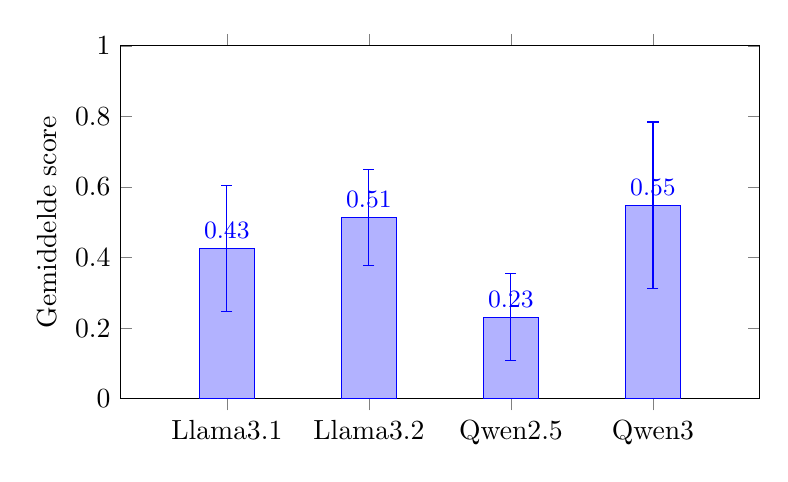
\begin{tikzpicture}
        \begin{axis}[
            ybar,
            ymin=0,
            ymax=1,
            bar width=20pt,
            width=0.8\textwidth,
            height=0.5\textwidth,
            enlarge x limits=0.25,
            ylabel={Gemiddelde score},
            symbolic x coords={Llama3.1,Llama3.2,Qwen2.5,Qwen3},
            xtick=data,
            nodes near coords,
            nodes near coords align={vertical},
            every node near coord/.append style={font=\small}
            ]
            \addplot+[
            error bars/.cd,
            y dir=both,
            y explicit
            ] coordinates {
                (Llama3.1,0.426) +- (0,0.178)
                (Llama3.2,0.514) +- (0,0.136)
                (Qwen2.5,0.231) +- (0,0.124)
                (Qwen3,0.548)   +- (0,0.236)
            };
        \end{axis}
    \end{tikzpicture}
    \caption{Gemiddelde score per model over de vier categorieën, met foutbalken die de standaarddeviatie weergeven. Llama3.2 vertoont de meest consistente prestaties, terwijl Qwen3 het hoogste gemiddelde behaalt maar met grotere spreiding.}
    \label{fig:gemiddelde_score_per_model_met_sd}
\end{figure}

\section{Evaluatie 2: Hallucinaties}

Bij deze test kreeg ieder model een set van vijf vragen voorgeschoteld. Geen van deze vragen komt voor in de documentatie. De antwoorden van de verschillende modellen zijn te raadplegen in bijlage \ref{hallucinatie-resultaten}. Dit heeft als doel om na te gaan welke modellen tekenen vertonen van hallucinaties en welke niet. 
\\[1em]
De vragenlijst is als volgt:

\begin{enumerate}
    \item Voor welke dienst is Jan Cabooter verantwoordelijk?
    \item Wat is de maximale bestandsgrootte (in MB) die via de repush voor RV kan worden verstuurd?
    \item Wat is de kost voor een Nationality change?
    \item Wat is de technical resource voor DQSS?
    \item Wat is het maximum aantal documenten die kunnen geraadpleegd worden bij myminfin
\end{enumerate}

\begin{table}[H]
    \begin{tabular}{|l|c|c|c|c|}
        \hline
        \textbf{Vraag} & \textbf{Llama3.1} & \textbf{Llama3.2} & \textbf{Qwen2.5} & \textbf{Qwen3} \\
        \hline
       Vraag 1 & Nee & Ja & Nee & Nee \\
       Vraag 2 & Nee & Ja & Ja & Ja \\
       Vraag 3 & Ja & Nee & Nee & Nee \\
       Vraag 4 & Nee & Ja & Nee & Nee \\
       Vraag 5 & Nee & Ja & Nee & Nee \\
        \hline
    \end{tabular}
    \caption{Resultaten hallucinatie test per model bij vragen die niet in de documentatie voorkomen (Ja = hallucinatie, Nee = geen hallucinatie). Uit de resultaten blijkt dat voornamelijk Llama3.2 frequent hallucinaties vertoont, terwijl de andere modellen dit nauwelijks doen.}
\end{table}

\noindent\textbf{Samenvatting:}  
\begin{table}[H]
    \begin{tabular}{|l|c|}
        \hline
        \textbf{Model} & \textbf{Hallucinatie (\%)} \\
        \hline
        Llama3.1 & 1/5 (20\%) \\
        Llama3.2 & 4/5 (80\%) \\
        Qwen2.5  & 1/5 (20\%) \\
        Qwen3    & 1/5 (20\%) \\
        \hline
    \end{tabular}
    \caption{Samenvatting hallucinatie test. Het percentage geeft aan hoe vaak een model hallucinaties vertoonde. Opvallend is dat Llama3.2 met 80\% veruit het vaakst hallucinaties genereerde, terwijl de andere modellen dit slechts in 20\% van de gevallen deden.}
\end{table}

Uit de resultaten blijkt dat Llama3.2 in 80\% van de gevallen hallucinaties vertoonde, terwijl de overige modellen dit slechts in 20\% van de gevallen deden.

\subsection{Bespreking van de resultaten}

De modellen Qwen3, Qwen2.5 en Llama3.1 vertoonden geen tekenen van hallucinaties. Ze hielden zich goed aan de instructie om geen extra informatie te verzinnen en zich uitsluitend te baseren op de gegevens die in de opgehaalde documenten stonden. Wel ondervond elk van deze modellen problemen bij het beantwoorden van één specifieke vraag. Na nader onderzoek bleek dat, wanneer het model de vraag in het Frans herschreef, de tool call niet altijd correct functioneerde. Het is niet meteen duidelijk waarom dit gebeurde, maar bij de andere vragen traden er bij deze modellen geen hallucinaties op.
\\[1em]
Llama3.2 daarentegen maakte meerdere keren aannames en verzon informatie die niet in de documentatie stond. Dit is uiteraard onwenselijk en kan verstrekkende gevolgen hebben voor de medewerkers die de support uitvoeren. Zeker wanneer zij deze informatie als waarheidsgetrouw beschouwen.

\subsubsection{Relevantie voor echte toepassingen}
%Hoe cruciaal is dit type vraag in de praktijk?

Aangezien de opgeleverde informatie wordt gebruikt voor het behandelen van specifieke IT-vragen van burgers over MyMinfin, is het van groot belang dat de modellen geen hallucinaties vertonen. Zelfs wanneer het model uitsluitend informatie levert aan de supportmedewerker, is het essentieel dat deze informatie waarheidsgetrouw is. Op zijn minst moet het model bij twijfel expliciet aangeven dat de benodigde informatie niet beschikbaar is. Op basis van deze test kan Llama3.2 niet realistisch worden ingezet.

\section{Evaluatie 3: Triviale vraagstelling}

Tijdens deze test kreeg ieder model een reeks van vijf triviale vragen voorgelegd. De resultaten werden bepaald door de stacktrace van ieder model te analyseren. Op die manier werd vastgesteld of het model de vraag direct beantwoordde of eerst onnodig RAG uitvoerde. Voor meer details kan bijlage \ref{triviale-vragen-resultaten} geraadpleegd worden.
\\[1em]
De vragenlijst is als volgt:

\begin{enumerate}
    \item Hallo hoe gaat het?
    \item Hoeveel dagen zitten er in een week?
    \item Wat is 2 + 2?
    \item In welk land ligt Parijs?
    \item Hoeveel minuten zitten er in een uur?
\end{enumerate}

\begin{table}[H]
    \centering
    \begin{tabular}{|l|c|c|c|c|}
        \hline
        \textbf{Vraag} & \textbf{llama3.1} & \textbf{llama3.2} & \textbf{Qwen2.5} & \textbf{Qwen3} \\
        \hline
        Hallo hoe gaat het? & Nee & Nee & Ja & Ja \\
        Hoeveel dagen zitten er in een week? & Nee & Nee & Ja & Ja \\
        Wat is 2 + 2? & Nee & Nee & Ja & Ja \\
        In welk land ligt Parijs? & Nee & Nee & Ja & Ja \\
        Hoeveel minuten zitten er in een uur? & Nee & Nee & Ja & Ja \\
        \hline
    \end{tabular}
    \caption{Resultaten van het correcte gebruik van de graaf per model bij triviale vragen waarbij verwacht wordt dat een direct antwoord wordt gegeven zonder gebruik van RAG. Er is een duidelijk onderscheid tussen de Llama-modellen en Qwen-modellen. De Llama-modellen raadplegen bij iedere vraag de vectordatabase terwijl de Qwen-modellen dit achterwege laten zoals wordt verwacht bij triviale vragen.}
    
\end{table}

\noindent\textbf{Samenvatting:}  
\begin{table}[H]
    \begin{tabular}{|l|c|}
        \hline
        \textbf{Model} & \textbf{Correct (\%)} \\
        \hline
        Llama3.1 & 0/5 (0\%) \\
        Llama3.2 & 0/5 (0\%) \\
        Qwen2.5  & 5/5 (100\%) \\
        Qwen3    & 5/5 (100\%) \\
        \hline
    \end{tabular}
    \caption{Samenvatting van correct gebruik van de graaf per model. Qwen2.5 en Qwen3 volgden in alle gevallen het verwachte gedrag terwijl Llama3.1 en Llama3.2 dit niet deden.}
\end{table}

Uit de resultaten blijkt dat Qwen2.5 en Qwen3 alle triviale vragen direct beantwoordden, terwijl Llama3.1 en Llama3.2 het omgekeerde deden.

\subsection{Bespreking van de resultaten}
%Verwachtte je een foutloos resultaat?
De resultaten waren in dit geval vrij duidelijk. De twee Llama-modellen slaagden er niet in onderscheid te maken tussen triviale en niet-triviale vragen. Dit leidde ertoe dat zij bij elke vraag het volledige ophaalproces uitvoerden. De twee Qwen-modellen daarentegen gaven direct antwoord op de triviale vragen. Met andere woorden: het contrast tussen de Qwen- en Llama-modellen was tijdens deze test aanzienlijk.
\\[1em]
Hoewel dit niet direct invloed heeft op de inhoudelijke correctheid van de antwoorden, heeft het wel gevolgen voor de performantie van de toepassing. Bij niet-triviale vragen duurt het beantwoorden aanzienlijk langer bij de Llama-modellen dan bij de Qwen-modellen. Voor een consistente en snelle werking van de PoC zijn de Qwen-modellen daardoor beter geschikt dan de Llama-modellen.
%Kunnen deze fouten vermeden worden met betere prompting?


\section{Samenvatting}
%Doel: Alles samenbrengen en overkoepelend reflecteren.
In deze vergelijkende studie werden vier modellen getest op drie verschillende manieren. Met name het beantwoorden van vragen op basis van opgehaalde documentatie, het behandelen van vragen die niet in de documentatie voorkwamen en het omgaan met triviale vragen. Elk model werd bij iedere deeltest beoordeeld op zijn prestaties.
\\[1em]
Op basis van deze testen kan worden geconcludeerd dat Qwen3 het beste model is in deze vergelijkende studie. In de eerste test behaalde het model twee keer de hoogste score en één keer de op één na hoogste score. Daarnaast vertoonde het model geen hallucinaties en ging het op een correcte manier om met triviale vragen. Met andere woorden is dit het enige model dat voor alle testen aan de verwachtingen voldeed. Op basis van deze resultaten kan worden geconcludeerd dat Qwen3 binnen deze PoC de meest betrouwbare prestaties leverde.
\\[1em]
De PoC met het Qwen3-model dekt de meeste noden die in de behoeften analyse naar boven kwamen. Ten eerste gaat het model goed om met meertaligheid. Er werden hieromtrent geen problemen vastgesteld. Het model slaagde er consistent in om te antwoorden in de taal van de gebruiker. 
\\[1em]
Daarnaast gaf het model aan wanneer het onvoldoende kennis had om een vraag te beantwoorden. Dit is van groot belang, aangezien het anders tot foutieve antwoorden kan leiden. Dit resultaat sluit aan bij de hoge score voor Faithfulness die Qwen3 behaalde. Wanneer het model een antwoord genereerde, vermeldde het bovendien vaak de bron van de informatie, wat positief is omdat de gebruiker de informatie op die manier kan verifiëren.  
\\[1em] 
Een aantal van de behoeften zijn niet vervuld. Een concreet voorbeeld hiervan is de afwezigheid van een volwaardige chatfunctionaliteit binnen de PoC.